\section{Real terrain: SRTM lines over the Sierra Nevada}\label{sec:realdem}

The scenes of the previous sections are synthetic. To check the joint reconstruction over the whole line on real relief,
azimuth lines were cut from the SRTM \SI{3}{\arcsecond} DEM (about \SI{90}{m}, WGS\,84) \cite{Farr2007srtm} over the
Sierra Nevada (California), using the file \texttt{raster/srtm90.tif} of \texttt{github.com/opengeos/data}. Every result is
still one azimuth line (1-D): a straight \SI{47}{km} profile of the DEM, sampled every \SI{90}{m} and interpolated linearly
between samples. The heights are taken relative to the mean height of the line, which is the reference height of the
processing. Point targets of unit amplitude are placed on the terrain, the four channels are simulated with
$\bxt=[0,300,119.8,100.5]$\,\si{m} (channel~0 on the transmitter), and the joint reconstruction receives the same SRTM
profile as its DEM, never the targets. The metric is the highest ambiguity of \cref{sec:metric}; the reference is the
monostatic full-rate line of the same scene. The script is \texttt{sata1d\_code/joint\_cases/real\_dem/run\_real\_dem.py}
and the figures are made by \texttt{real\_dem\_figures.py} in the same folder.

\begin{figure}[htbp]
\centering
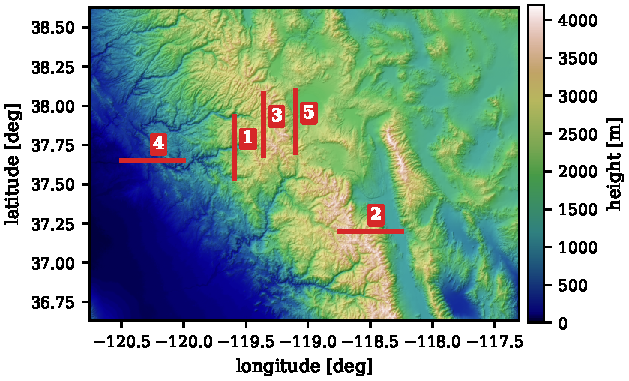
\includegraphics[width=0.72\linewidth]{figures/realdem_map.pdf}
\caption[SRTM DEM of the Sierra Nevada and the five named lines]{SRTM \SI{3}{\arcsecond} DEM of the Sierra Nevada with
the five named lines of \cref{tab:realdem} (red, \SI{47}{km} each). The map only shows where the lines come from: every
result is computed on one line.}
\label{fig:realdem-map}
\end{figure}

\begin{table}[htbp]
\centering
\caption[Real terrain: the five named lines]{The five named SRTM lines with five targets each (at
$x=-5.0,-2.4,0,2.6,5.3$\,\si{km}, chosen so that no ghost at $\pm X$ or $\pm2X$ falls on another target). Highest ambiguity
in dB; the reference is \SI{-41.6}{dB} on every line (sidelobes of the neighbouring targets inside the ghost windows).}
\label{tab:realdem}
\small
\begin{tabular}{@{}l l c c c@{}}
\toprule
Line & Direction & Terrain height [m] & No correction [dB] & Joint [dB] \\
\midrule
1 Yosemite Valley           & north--south & 1213--2893 & $-5.7$ & $-41.5$ \\
2 Eastern Sierra escarpment & west--east   & 1198--4053 & $-8.2$ & $-41.5$ \\
3 High Sierra, Tuolumne     & north--south & 2351--3635 & $-6.0$ & $-41.6$ \\
4 Western foothills         & west--east   & 52--932    & $-6.1$ & $-41.4$ \\
5 Mono basin                & north--south & 1948--3432 & $-6.2$ & $-41.0$ \\
\bottomrule
\end{tabular}
\end{table}

\Cref{fig:realdem-yosemite,fig:realdem-escarpment,fig:realdem-highsierra} show three of the lines. Without correction every
target leaves ghosts at $\pm X$ and $\pm2X$ ($X=\SI{6.23}{km}$) between \SI{-8.2}{dB} and \SI{-5.7}{dB}; the joint
reconstruction brings all of them to the level of the reference, within \SI{0.6}{dB} on the five lines
(\cref{tab:realdem}). The Yosemite line has steep valley walls (about \SI{1700}{m} of relief over a few kilometres), the
escarpment line goes from the Sierra crest down to the floor of Owens Valley (\SI{2800}{m}), and the High Sierra line has
many short slopes, so that the height, and with it the phase of every channel, changes every few hundred metres. None of
these is a difficulty for the joint reconstruction, because it applies the DEM phase at every position of the line.

\begin{figure}[htbp]
\centering
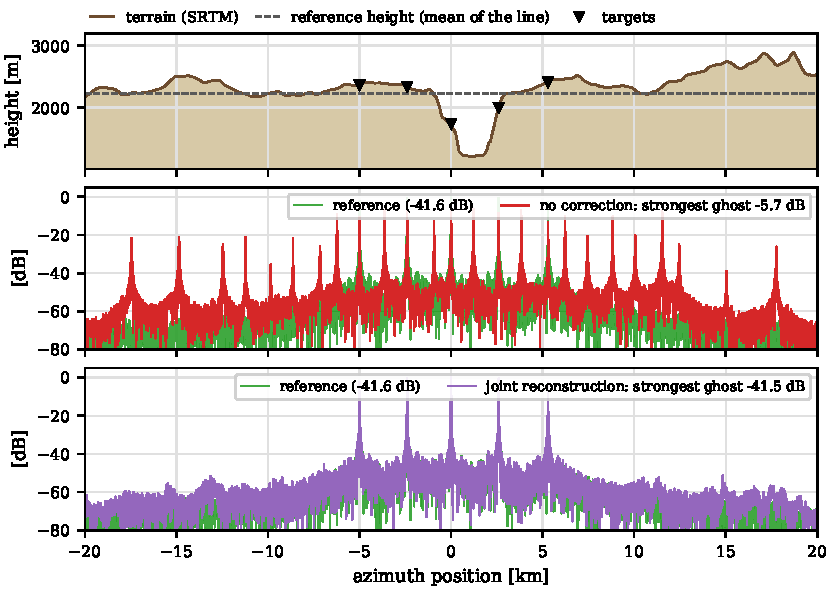
\includegraphics[width=\linewidth]{figures/realdem_lines5_yosemite.pdf}
\caption[Real terrain: Yosemite Valley]{Yosemite Valley (north--south, line~1). Top: SRTM profile, reference height and the
five targets. Middle and bottom: focused line in dB relative to the peak of the reference, without correction and with the
joint reconstruction; the reference (green) is drawn below both.}
\label{fig:realdem-yosemite}
\end{figure}

\begin{figure}[htbp]
\centering
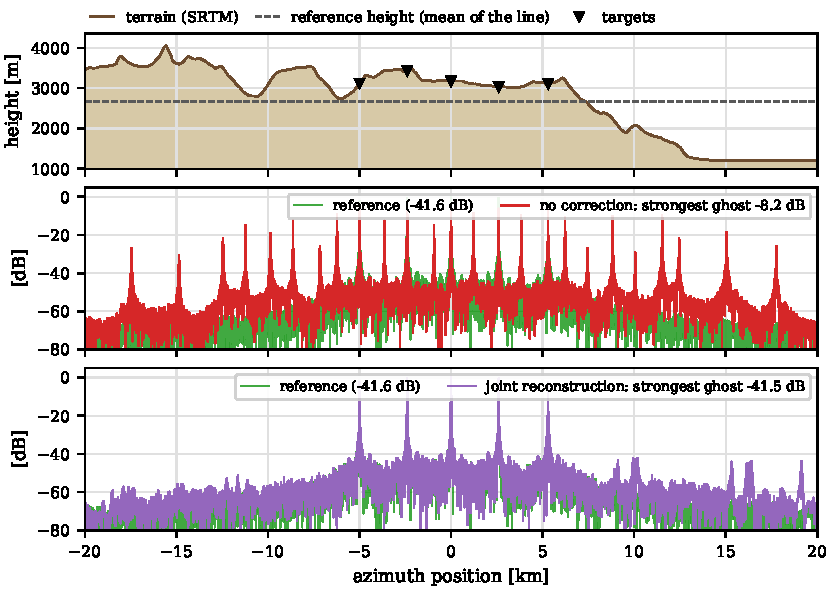
\includegraphics[width=\linewidth]{figures/realdem_lines5_escarpment.pdf}
\caption[Real terrain: eastern Sierra escarpment]{Eastern Sierra escarpment (west--east, line~2), from the crest to the floor
of Owens Valley; same layout as \cref{fig:realdem-yosemite}.}
\label{fig:realdem-escarpment}
\end{figure}

\begin{figure}[htbp]
\centering
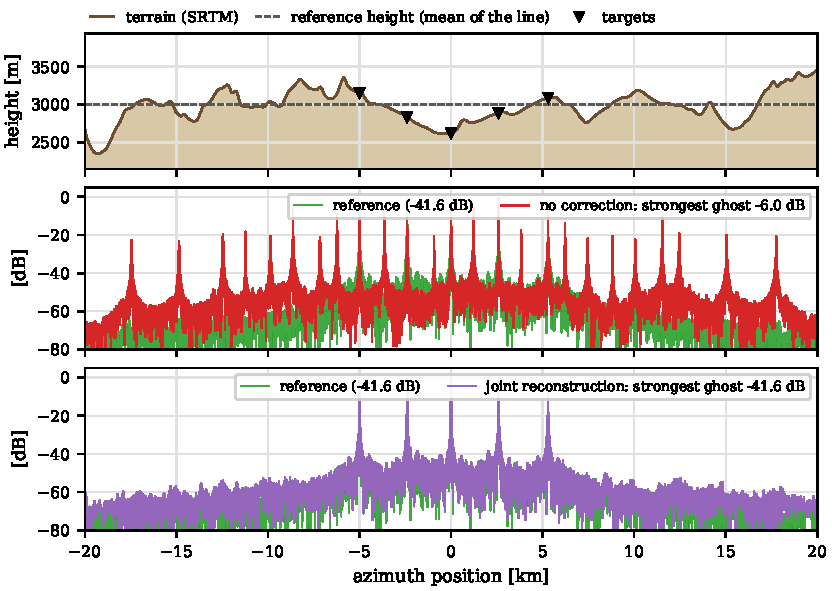
\includegraphics[width=\linewidth]{figures/realdem_lines5_highsierra.pdf}
\caption[Real terrain: High Sierra]{High Sierra near Tuolumne (north--south, line~3): rugged peaks and valleys; same layout
as \cref{fig:realdem-yosemite}.}
\label{fig:realdem-highsierra}
\end{figure}

\Cref{fig:realdem-zoom} zooms on the Yosemite target that is farthest from the reference height (on the valley floor,
\SI{487}{m} below it). Without correction the peak is \SI{4.4}{dB} low and \SI{29.7}{\degree} off, because part of its
energy went to the ghosts; the ghost at $+X$ is at \SI{-10.2}{dB}. With the joint reconstruction the peak equals the
reference within \SI{0.01}{dB} and \SI{0.02}{\degree}, and the ghost drops to \SI{-43.1}{dB}, below the sidelobes of the
reference around it.

\begin{figure}[htbp]
\centering
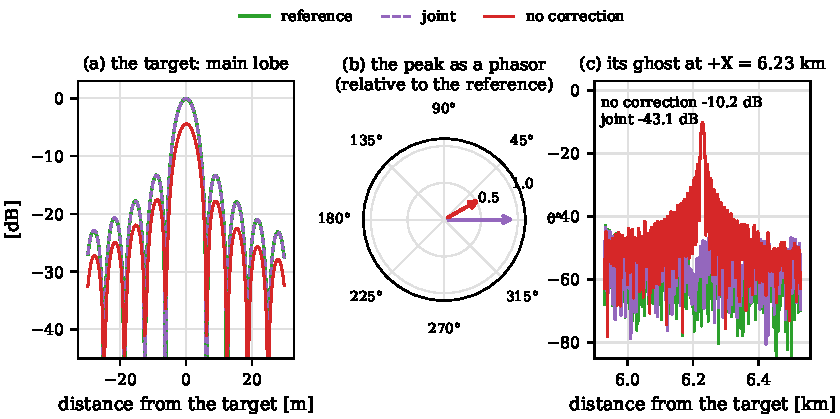
\includegraphics[width=\linewidth]{figures/realdem_zoom.pdf}
\caption[Real terrain: zoom on one target]{Yosemite, valley-floor target \SI{487}{m} below the reference height. (a) Main
lobe; the joint line lies on the reference. (b) Complex peak relative to the reference. (c) The window of its ghost at
$+X$. All levels in the processed band $\Ba$, relative to the peak of the reference.}
\label{fig:realdem-zoom}
\end{figure}

\paragraph{Many targets.} With 20 targets every \SI{750}{m} (from \SIrange{-7.1}{7.1}{km}) every ghost falls between
two targets, and the highest ambiguity is the worst of 80 ghost windows per line. The reference reaches only
\SI{-32.0}{dB} here, from the sidelobes of the neighbours inside the windows. Without correction the five lines give
\SIrange{-5.7}{-5.1}{dB}; the joint reconstruction gives \SIrange{-31.5}{-28.1}{dB}, within \SI{4}{dB} of the reference
(\cref{fig:realdem-20}).

\begin{figure}[htbp]
\centering
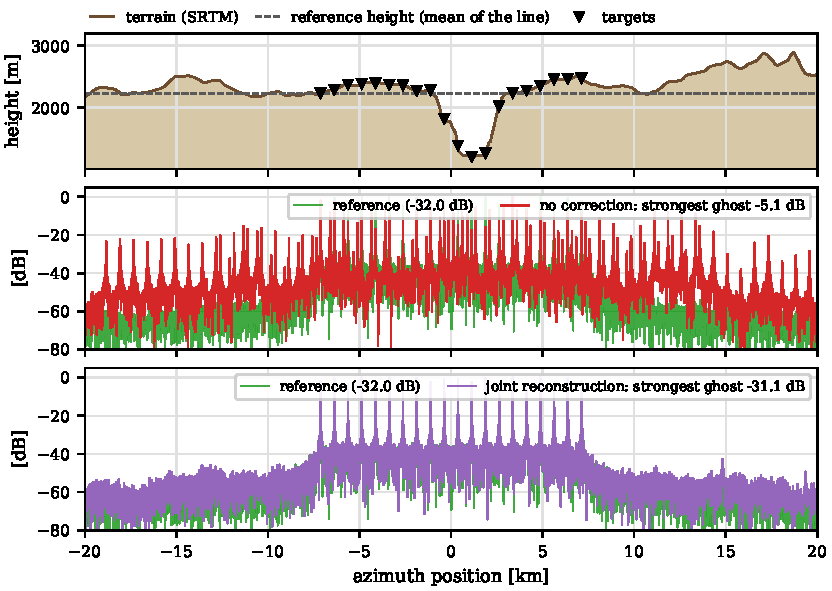
\includegraphics[width=\linewidth]{figures/realdem_lines20_yosemite.pdf}\\[4pt]
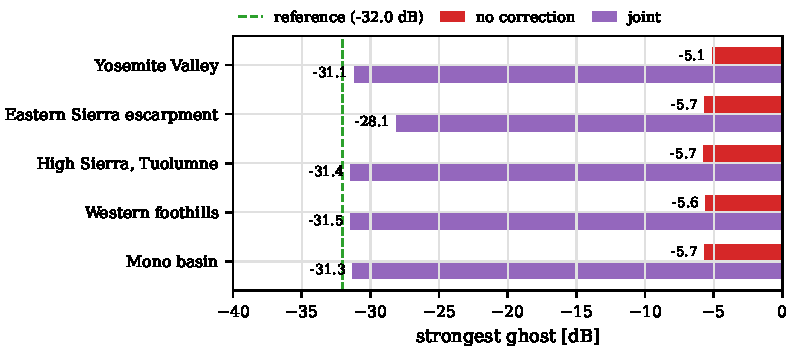
\includegraphics[width=0.78\linewidth]{figures/realdem_lines20_summary.pdf}
\caption[Real terrain: 20 targets per line]{Top: Yosemite line with 20 targets every \SI{750}{m}; same layout as
\cref{fig:realdem-yosemite}. Bottom: highest ambiguity of the five lines with 20 targets each.}
\label{fig:realdem-20}
\end{figure}

\paragraph{200 random lines.} To avoid choosing the lines by hand, 200 lines were drawn at random over the whole DEM
(random centre and direction, the full \SI{47}{km} inside the raster), with the five targets of \cref{tab:realdem}. The
relief of a line reaches \SI{2930}{m}; half of the lines use $\bxt=[0,300,119.8,100.5]$\,\si{m} and half
$\bxt=[0,134.9,20.5,8.3]$\,\si{m} (largest \SI{135}{m}). \Cref{fig:realdem-random} gives the result: the median highest
ambiguity goes from \SI{-8.3}{dB} without correction to \SI{-41.5}{dB} with the joint reconstruction (reference
\SI{-41.6}{dB}), a median gain of \SI{33}{dB}. In the 192 lines with more than \SI{200}{m} of relief the gain is at least
\SI{28}{dB} in \SI{92}{\percent} of them, and the joint reconstruction is within \SI{10}{dB} of the reference in 199 of the
200 lines. It is never worse than no correction by more than \SI{0.03}{dB}; that happens only on a flat line
(\SI{16}{m} of relief), where both are already at the reference. The gain grows with the relief, because the uncorrected
ghosts grow with it while the joint result stays at the reference.

\begin{figure}[htbp]
\centering
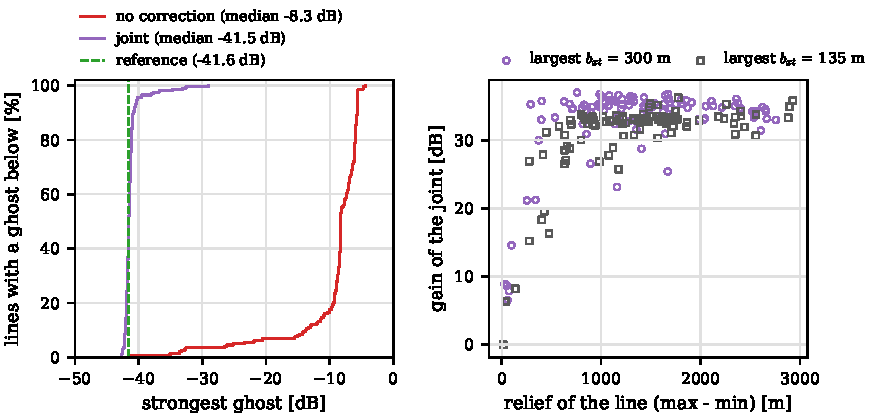
\includegraphics[width=\linewidth]{figures/realdem_random200.pdf}
\caption[Real terrain: 200 random lines]{200 random SRTM lines over the Sierra Nevada, five targets each. Left: cumulative
distribution of the highest ambiguity. Right: gain of the joint reconstruction over no correction against the relief of the
line, for the two baseline sets.}
\label{fig:realdem-random}
\end{figure}

These runs share the limits of the rest of the chapter: the DEM given to the reconstruction is exactly the terrain of the
simulation (with DEM errors the floor rises as in \cref{fig:demerror}), the antenna pattern is the simulated one, and each
line is processed in 1-D.
